\chapter{Experimental Setup}
This chapter describes the experimental setup of this thesis, including the data collection and preparation process, the retrieval pipeline development and how the LLM answers are generated.

\section{Overview}\label{sec:overview}
The final goal of this project is to have a pipeline with which the answers of different LLMs can be ranked, in comparison to human answers.
This means, we first need a dataset, consisting of questions as well as human answers to these questions.
Those human generated answers need to be ranked according to how well they answer the given question.
Then, we need to develop a retrieval pipeline, which is able to rank the answer to a given question in accordance to the ranking of the human answers.
Finally, the answers generated by different LLMs can be ranked using the developed retrieval pipeline.
\\
This allows us to compare long form question answering capabilities between different LLMs or between different prompting strategies for the same LLM, by comparing the ranking positions of the generated answers.
\\\\
To be able to do this, we first need to collect a suitable dataset, since a benchmark like this has not been formulated before.
Then, different retrieval methods have to be compared on the dataset, to find the best performing one.
Finally, the LLMs have to be selected, and the answers generated by them have to be ranked using the best retrieval method.
\\
This process is described in detail in the following sections.

\section{Data Collection and Preparation}\label{sec:dataset}
The used dataset is based on the test set of the CLEF eHealth 2021 dataset \cite{goeuriot:2021:Consumer}.
It was originally intended to evaluate the ability of retrieval systems to provide credible, readable and relevant answers to laypersons' health questions.

\subsection{CLEF eHealth 2021 Dataset}
The test set consists of 55 health related queries which either stem from Reddit or Google search trends.
While the Reddit-sourced queries are well-formulated questions about specific health topics, the queries from Google search trends are not necessarily phrased as questions but rather as classical keyword-based search queries.
\\
\\
In addition to the queries, the dataset includes a collection of web documents and social media content.
The web documents were mainly obtained from the CommonCrawl archive, containing a diverse range of 600 domains.
This list of domains was created by executing medical queries via Microsoft Bing API and was augmented by adding known reliable and unreliable health-related websites.
The dataset was expanded by incorporating social media comments and posts from Reddit and Twitter.
These were collected by manually generating search queries based on 150 pre-selected health topics and retrieving relevant posts and comments from these platforms, after posting the queries.
\\
To get evaluations in each of the three categories (relevance, readability and credibility), each query was assigned 250 documents based on rank-biased precision (RBP)-based Method A~(\cite{moffat:2008:Rank}).
RBPA is a method for choosing which documents from a pool of documents to select for evaluation by human annotators.
The pool of documents in this case is the collection of web documents and social media content returned by the participating teams of the shared task, as well as the organizer's baseline systems.
From this, documents are evaluated based on their rank in different runs, and then scored according to the three different metrics.
A more detailed description of the pooling method can be found in \cite{lipani:2017:Fixed}.
\\
After the 250 documents per query are selected, the documents are evaluated by humans for credibility, readability and relevance.
In total, there are 26 annotators, each annotating documents for between 1 and 4 queries completely.
The annotators were not medical experts, but received written training material.
In the end, three annotations were made for  a total of $11 357$ unique documents.
This differs from the total amount of annotations in each metric which is $12 500$, since some documents were annotated multiple times but for different queries.
\\
The annotations for relevance and readability are in the categories 0 (not relevant/readable), 1 (somewhat relevant/readable) and 2 (highly relevant/readable).
For scoring credibility, a category 3 exists, which is also interpreted as highly credible.
A reasoning for this additional ranking score for credibility is not given in the original paper.
\\\\
The following sections describe how the dataset was collected and prepared for the experiments in this thesis.
\subsection{Dataset Collection}
There are two ways of accessing the CLEF eHealth 2021 dataset.
\\
Option one is to download the indexed collection directly.
This index does not contain the full text of the documents, so it can not be used to compare the original documents against newly generated answers.
\\
The second option is to download all documents individually, given their IDs.
This is in easily done in theory, by using the provided scripts in the organizer's GitHub repository\footnote{\url{https://github.com/CLEFeHealth/CHS-2021}}.
Scripts are provided to download the documents from the CommonCrawl archive, as well as the social media content directly over the respective APIs.
\\
Unfortunately, with Twitter shutting down their free tier of the API, in the beginning of April 2023, this is now only possible with a prohibitively expensive paid tier.
\\
For Reddit, those API changes followed just a few months later, making it impossible to download the social media content from Reddit as well.
Even tough we started downloading some Reddit content before those changes, the already slow access to the Reddit data did not allow for downloading all content in time.
\\
This was unfortunate timing, but since the organizers of the CLEF eHealth task reported in their paper that the human credibility assessments of social media documents were significantly lower than those of web documents, we decided to only use the web documents for our dataset.
The web documents are easily accessible via the CommonCrawl archive.
\\
\\
Before accessing all relevant documents from the CommonCrawl archives, the list of documents is filtered to only include documents which are annotated for at least one query.
Discarding all documents from Reddit and Twitter, as well as web documents which are not assessed for any query, results in a total of $6692$ documents downloaded from the CommonCrawl archive using a slightly modified version of the provided script.
This provides us with WARC files for the relevant documents.
\\
Since all social media content is discarded, the number of queries for which documents are available is reduced to 50, since of the total 55 queries, 5 queries only have social media content associated with them.

\subsection{Preprocessing}
The files in the WARC format contain the full HTML of the web documents.
Before being able to compare the content to the generated answers, the HTML is extracted from the documents.
HTML elements containing fewer than 50 characters in the elements body are discarded, assuming they are not relevant for the content of the document (e.g. fields of navigation bars).
Then, the plain text is extracted using the ChatNoir Resiliparse Library\footnote{\url{https://resiliparse.chatnoir.eu/en/stable/}}.
\\
The final dataset now consists of 50 queries, each of which has between 39 and 249 documents associated with it that are evaluated for relevance, readability and credibility.


\section{Retrieval Pipeline Development}
In this section, the implementation of the different retrieval pipelines is discussed.
The baseline models (DPH and TF-IDF), as well as the ColBERT version 1 and the monoT5/duoT5 based pipelines are implemented in the PyTerrier framework by \cite{pyterrier:2020:Declarative}, which is a Python API for the Terrier IR Platform~(\cite{macdonald:2012:From}).
The ColBERT version 2 pipeline is based on the original implementation provided by the authors\footnote{\url{https://github.com/stanford-futuredata/ColBERT}}.
\\
Those pipelines are all designed to retrieve the most relevant documents for a given query.
Since our dataset also contains annotations for readability and credibility, we also want to be able to retrieve documents based on those criteria.
To extend the retrieval pipelines for those metrics, we experiment with adding external scores to the retrieval process.
This is described in section \ref{sec:external-scores}.
\\

\subsection{Retrieval Setup}
The retrieval setup in this work differs from the usual retrieval setup, in which a large document collection is indexed, and then multiple queries are run against the index using different retrieval models.
In our case, we build separate indices for each query, containing only the documents that are evaluated for that query.
This ensures that each document that is retrieved for a query is also evaluated for that query.

\subsection{Baseline Models}
This section describes the implementation of the baseline models, namely DPH and TF-IDF.
For both models, the basic indexing function of PyTerrier is used, which indexes and preprocesses the documents.
Preprocessing is done with the default values, which includes the following operations:
\begin{itemize}
    \item{\textbf{Tokenization}, for splitting the text into individual words or tokens. The default PyTerrier tokenizer splits text on non-alphanumeric characters. Additional rules to discard tokens which are longer than 20 characters, contain more than 4 digits, or contain the same character more than 3 times in a row are applied. All tokens are also converted to lowercase.}
    \item \textbf{Stopword removal}, to remove tokens that do not contain information about the content. We use the default PyTerrier stopword list.
    \item \textbf{Stemming}, to remove the different endings a token can have, leaving only the root of the word. For this the Porter stemmer which is a rule-based stemmer is used.
\end{itemize}
The resulting inverted index contains all remaining tokens, and a mapping from each token to the documents in which it occurs.
\\
The two retrieval models TF-IDF and DPH are then applied using the default parameters.
More details about the models can be found in section \ref{sec:baseline-retrieval-models}.
\\
\\
Both models are tested with and without query expansion.
We use BO1 query expansion, which is a query expansion method that uses the documents retrieved by the original query to expand the query.
It adds terms from the retrieved documents to the original query based on informativeness, which is a measure of how frequently the term occurs in the documents compared to how frequently it occurs in the whole collection.
Terms that occur more frequently in the retrieved documents than in the collection are added to the query.
Afterwards, the expanded query is run against the index again, and the documents are ranked according to the new query.
\\
\\
\begin{figure}[tb]
    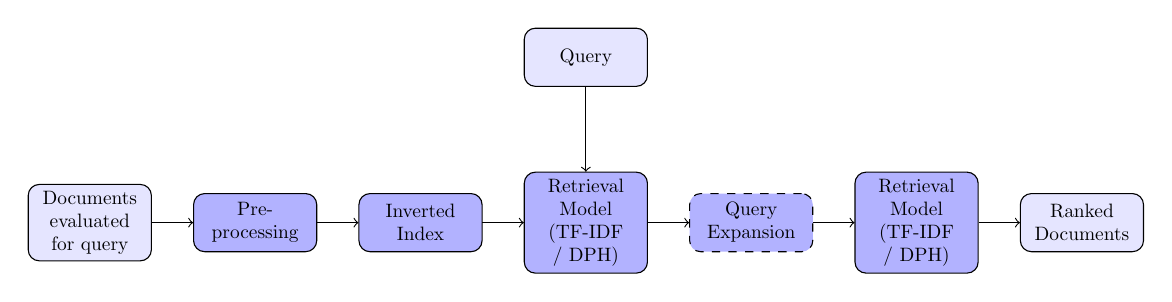
\begin{tikzpicture}[node distance=3cm, every node/.style={scale=0.7}]
    \tikzstyle{box} = [rectangle, draw, fill=blue!10,  text width=2cm, text centered, rounded corners, minimum height=3em]
    \tikzstyle{process} = [rectangle, draw, fill=blue!30,  text width=2cm, text centered, rounded corners, minimum height=3em]
    \node (docCol) [box] {Documents evaluated for query};
    \node (preprocess) [process, right of=docCol] {Pre-\\processing};
    \node (invertedindex) [process, right of=preprocess] {Inverted Index};
    \node (retrieval) [process, right of=invertedindex] {Retrieval Model (TF-IDF / DPH)};
    % query expansion with dotted line around
    \node (qe) [process, right of=retrieval, dashed] {Query Expansion};
    \node (reranking) [process, right of=qe] {Retrieval Model (TF-IDF / DPH)};
    \node (ranked) [box, right of=reranking] {Ranked Documents};
    \node (query) [box, above of=retrieval] {Query};

    \draw [->] (docCol) -- (preprocess);
    \draw [->] (preprocess) -- (invertedindex);
    \draw [->] (invertedindex) -- (retrieval);
    \draw [->] (retrieval) -- (qe);
    \draw [->] (qe) -- (reranking);
    \draw [->] (reranking) -- (ranked);
    \draw [->] (query) -- (retrieval);

    \end{tikzpicture}
\caption{Baseline retrieval pipeline, using either TF-IDF or DPH as retrieval model with optional query expansion. This retrieves and ranks evaluated documents for a given query.}
\label{fig:baseline-pipeline}
\end{figure}
The resulting pipeline is shown in figure \ref{fig:baseline-pipeline}.
This produces a ranked list of documents for each query, which can then be compared to the order of documents according to the human annotations.

\subsection{Transformer Models}
In addition to the baseline models, we also implement the transformer based models ColBERT version 1 and 2, as well as the monoT5 and duoT5 based models.
The implementation of ColBERT version 1 and the MonoT5/DuoT5 based models is done in PyTerrier, while the implementation of ColBERT version 2 is done in the original implementation provided by the authors.
\\\\
All of the models are based on a pre-trained model, which is at some point used to encode the query and the documents in differnet ways.
Both ColBERT versions are based on the BERT-base model, while the MonoT5 and DuoT5 based models are based on the T5 model.
The retrieval models themselves are fine-tuned on the MS MARCO passage ranking dataset~(\cite{bajaj:2016:MSMARCO}), a large scale dataset for passage retrieval.
\\
Transformer-based retrieval models usually require a first retrieval step using a less computationally expensive model like tf-idf, to reduce the number of documents that are fed to the transformer model.
Because in this thesis the retrieval dataset is small, the first retrieval step is omitted for all transformer-based models.

\subsubsection{ColBERT Version 1}
Using the ColBERT implementation for PyTerrier\footnote{\url{https://github.com/terrierteam/pyterrier_colbert}}, an end-to-end pipeline can be constructed from a pre-trained ColBERT model and a document collection.
In our testing, we use the pre-trained ColBERT checkpoint provided by the authors.
\\
The checkpoint can directly be loaded in the PyTerrier framework, and then used to retrieve documents from the collection.
All settings are left at their default values.

\subsubsection{MonoT5 and DuoT5}
Like the ColBERT implementation, the monoT5 and duoT5 implementations are also available in PyTerrier\footnote{\url{https://github.com/terrierteam/pyterrier_t5}}.
Pre-trained checkpoints based on the MS MARCO dataset are provided by the authors.
\\
The monoT5 pipeline uses the pre-trained checkpoint to encode each query with each of the associated documents.
From this encoding a score is calculated for each query-document pair, and the documents are ranked according to this score.
\\
The duoT5 pipeline is based on the monoT5 pipeline, but uses the duoT5 re-ranker to re-rank the top 10 documents retrieved by the MonoT5 pipeline.
Here, the pre-trained duoT5 checkpoint is used to encode the query and each possible pair of the top 10 documents, to determine which of the two documents is more relevant to the query.
Based on this order, the documents are re-ranked.
\\
Again, all parameters are left at their default values.

\subsubsection{ColBERT Version 2}
Unlike the other transformer based models, ColBERT version 2 is not available directly in PyTerrier.
Instead, we use the implementation provided by the authors of the model\footnote{\url{https://github.com/stanford-futuredata/ColBERT/tree/main}}.
\\
The implementation works with any pre-trained checkpoint for the ColBERT version 2 model, with the MS MARCO checkpoint being downloaded by default.

\subsection{External scores for Readability}\label{sec:external-scores}
% TODO: Should we add readability and credibility from Huggingface? 
To improve retrieval performance for the readability, we experiment with adding pre-computed external scores to the retrieval process.

To estimate readability of the documents in the dataset, different scores are calculated for each document.
\\
The first score is the Flesch Reading Ease (FRE) score devised by \cite{kincaid:1975:Derivation}, which is a score between 0 and 100, with higher scores indicating easier to read text.
It is calculated using the following formula, based on average sentence length (ASL) and average number of syllables per word (ASW):
\begin{equation}
    FRE = 206.835 - (1.015 \times ASL) - (84.6 \times ASW)
\end{equation}
We use the implementation provided by the textstat library\footnote{\url{https://pypi.org/project/textstat/}}.
\\
This library also provides the second score, which is an aggregate of multiple similar scores, like the FOG score, the SMOG score and the Coleman-Liau Index.
Those scores are all based on different text statistics, like the number of syllables per word, the number of words per sentence or the number of characters per word.
More details about the different scores can be found in the documentation of the textstat library.

\section{Generating LLM Responses}
This section details which LLMs are selected for the experiments, and how the responses are generated.
We also describe the different prompting strategies that are used to generate the responses.

\subsection{Selection of Language Models}
We select multiple LLMs for our experiments, which differ in number of parameters, amount and type of training data and the type of pre-training and fine-tuning.

\subsubsection{GPT-2}
As a simple baseline and to investigate how an increased number of parameters affects the ranking results, we select different sizes of the GPT-2 model, namely the base, medium, large and XL versions.
Those models only differ in the number of parameters, which are 124M, 355M, 774M and 1.5B respectively, while training objective and the training data are the same for all of the models.
The dataset used for pre-training is the WebText dataset, which consists 40GB of web text, which is scraped from URLs shared on Reddit that received at least 3 upvotes.
Other than this pre-training, the models are not fine-tuned to any specific task.

\subsubsection{Models optimized for dialog}\label{sec:dialog-models}
Dialog optimized models are fine-tuned for the task of interacting with a human in a dialog, usually as a chatbot.
This is currently the use case of LLMs that comes closest to the task of long form question answering, so including models optimized for dialog is a natural choice.
To make a model suitable for directly interacting with humans, different fine-tuning objectives are used in which the behavior of the model is aligned with the expectations of the human.
\\
The importance of this alignment is shown by \cite{ouyang:2022:Training}, who show that answers of their instruction-tuned model InstructGPT are prefered by humans compared to outputs by a model with over 100 times the number of parameters, but without any fine-tuning.
\\
We select the following models:
\\\\
The \textbf{Falcon} family of models, which was released in 2023 on HuggingFace\footnote{\url{https://huggingface.co/blog/falcon}}.
At time of writing, there are three models sizes available, 7B, 40B and 180B parameters, each as a foundation model or as an instruction-tuned model.
For our testing, we only use the small 7B instruction-tuned model.
\\
According to the HuggingFace model card, the model is pre-trained on the RefinedWeb dataset by \cite{penedo:2023:The} and then fine-tuned on the GPTeacher\footnote{\url{https://github.com/teknium1/GPTeacher}}, GPT4All\footnote{\url{https://github.com/nomic-ai/gpt4all}} and Baize~(\cite{xu:2023:Baize}) datasets.
GPTeacher and GPT4All are both datasets of prompt-response pairs, while Baize is a dataset based on self-chats by ChatGPT, which have been seeded by questions from Quora, StackOverflow and MedQuAD.
\\
Unfortunately, the authors do not detail exactly how the data was used to fine-tune the model, as a scientific paper is still yet to be released.
\\
\\
\textbf{Llama 2}, a model introduced in 2023 by \cite{touvron:2023:Llama}.
It is available through the HuggingFace library, after agreeing to the terms of use posed by Meta.
It comes in three sizes, 7B, 13B and 70B parameters.
For each of the sizes, the base language model, and a fine-tuned version for chat is available.
In our testing, we use the fine-tuned version in both the 7B and 13B sizes, since the 70B parameter model is too large to fit on the available hardware.
\\
To create the chat model, the base model is first tuned using supervised fine-tuning, where the model is trained on a dataset of prompt-response pairs, which are all written by humans.
The model is then tuned to generate the response, provided the prompt.
\\
The next step is Reinforcement Learning with Human Feedback (RLHF), by which the model is aligned to human preferences. 
To generate a training set, humans are tasked to evaluate which of two generated responses to a given prompt they prefer.
Based on that data, a reward model is trained, which can then evaluate generated responses on a large scale.
The model is then fine-tuned to maximize the reward given by the reward model.
\\
The RLHF training is done over multiple iterations, continuously improving the reward model and the chat model based on human feedback.
Additionally, they not only optimize for helpfulness of the generated response, but also evaluate for safety, instructing the model not to provide harmful content in that way.
\\
\\
\textbf{ChatGPT}, is the largest model we used, with 175B parameters. 
It was introduced by OpenAI in the end of 2022\footnote{\url{https://openai.com/blog/chatgpt/}}.
As a commercial product, it can only be accessed through the OpenAI API, which we did using the provided Python library.
\\
With OpenAI becoming more secretive about their models since starting to monetize them, the exact training data and fine-tuning procedure is not known.
In their blog post, they state that the model is a close sibling to the InstructGPT model mentioned above.
This means the fine-tuning procedure is likely similar to the one described by \cite{ouyang:2022:Training}, but with a larger model size.
The methods applied are similar to the ones used for the Llama 2 model, first using supervised fine-tuning, and then using RLHF to align the model with human preferences.
\\
\\
Table \ref{tab:language-models} gives an overview of all the used models, comparing parameter size pre-training and fine-tuning data, as well as fine-tuning methods.
In total, we use 8 different models, 4 of which are variants of GPT-2, while the others a different fine-tuned models for chat.
\begin{table}[tb]
\centering
\begin{tabularx}{\textwidth}{lllXXX}
\hline
\textbf{Model} & \textbf{Params} & \textbf{Release} & \textbf{Pre-training Data} & \textbf{Fine-tuneing Data} & \textbf{Fine-tuneing Methods} \\
\hline
GPT-2 Base    & 124M & \multirow{4}{*}{2019} & \multirow{4}{*}{WebText} & \multirow{4}{*}{-} & \multirow{4}{*}{-} \\
GPT-2 Medium  & 355M &                      &                          &  &  \\
GPT-2 Large   & 774M &                      &                          &  &  \\
GPT-2 XL      & 1.5B &                      &                          &  &  \\
\hline
Falcon 7B              & 7B      & 2023 & RefinedWeb           & GPTeacher, GPT4All, Baize & SFT \\
\hline
Llama 2 7B & 7B    & \multirow{2}{*}{2023} & \multirow{2}{*}{Custom} & \multirow{2}{*}{Custom} & \multirow{2}{*}{SFT, RLHF} \\
Llama 2 13B   & 13B   &  &                        &                         &  \\
\hline
ChatGPT                & 175B   & 2022 & Custom                & Custom & Custom \\
\hline
\end{tabularx}
\caption{Comparison of evaluated Language Models. SFT = Supervised Fine-Tuning, RLHF = Reinforcement Learning with Human Feedback}\label{tab:language-models}
\end{table}

\subsection{Prompting approaches}\label{sec:prompting-approaches}
How a LLM is prompted to complete a task has a large impact on the quality of the generated response.
\cite{reynolds:2021:Prompt} show this in the context of translating French to English.
They compare the effect of three different prompting strategies on the 6.7 B and 13 B parameter versions of GPT-3:
\begin{enumerate}
    \item \textbf{Strategy 1}\\Q: What is the English translation of \textit{french\_sentence} A: \textit{translation}
    \item \textbf{Strategy 2}\\French: \textit{french\_sentence}\\English: \textit{translation}
    \item \textbf{Strategy 3}\\A French phrase is provided: \textit{french\_sentence}\\
    The masterful French translator flawlessly translates the phrase
into English: \textit{translation}
\end{enumerate}
where \textit{french\_sentence} is replaced by the sentence to be translated before prompting the model, which then generates the \textit{translation}.
According to their results in the BLEU metric, the first prompting strategy is outperformed by the other two.
Of those two, the third one performs better on the smaller 6.7B model, while on the 13B model, they perform  about equally well.
Table \ref{tab:fr-en-prompting} shows the large differences in the BLEU score between the different prompting strategies.
\begin{table}[tb]
\centering
\begin{tabularx}{\textwidth}{lXXX}
\hline
\textbf{Model} & \textbf{Strategy 1} & \textbf{Strategy 2} & \textbf{Strategy 3} \\
\hline
6.7B & 15.9 & 23.5 & 26.5 \\
13B & 18.7 & 33.3 & 32.9 \\
\hline
\end{tabularx}
\caption{BLEU scores for different prompting strategies for the 6.7B and 13B models of GPT-3, as reported by \cite{reynolds:2021:Prompt}}\label{tab:fr-en-prompting}
\end{table}
\\
Based on those results we use a similar approach of different prompting strategies for our experiments.
We use the following four strategies:
\begin{enumerate}
    \item \textbf{No Prompt:}\\ \textit{query}
    \item \textbf{QA Prompt:}\\ Q: \textit{query}\\A:
    \item \textbf{QuestionAnswer Prompt:}\\ Question: \textit{query}\\Answer:
    \item \textbf{MultiMedQA Promp:}\\ You are a helpful medical knowledge assistant. Provide useful, complete, and scientifically-grounded answers to common consumer search queries about health.\\Question: \textit{query}\\Complete Answer:
\end{enumerate}
where \textit{query} is replaced by the query to be answered.
Based on the results of \cite{reynolds:2021:Prompt}, we expect the generated answers based on the MultiMedQA prompt to rank highest, followed by the QuestionAnswer prompt.
To restrict the influence of random variations in the generated responses, we generate 10 responses for each query and model.
\\
\subsection{Generating Answers}
To generate answers for a given query, the query is passed to the LLM using one of the prompting strategies described above.
Most LLMs take additional parameters as input, which are used to guide the text generation process.
The following parameters are considered for the different models in our experiments:
\begin{itemize}
    \item \textbf{max new tokens}: This parameter defines the maximum number of new tokens to be generated by the LLM, limiting the length of the generated output.
    \item \textbf{temperature}: The temperature parameter controls the randomness in the generation process. A higher temperature value increases randomness in the output, while a lower value leads to more deterministic outputs.
    \item \textbf{top k}: This parameter sets a threshold for the number of most likely next tokens to consider at each step of generation, only allowing the model to choose from the top k tokens. A higher value for k will increase the diversity of the generated output, while a lower value will decrease diversity.
    \item \textbf{top p}:  Also called nucleus sampling, specifies a cumulative probability threshold. The model will only consider the smallest set of tokens whose cumulative probability does not exceed the threshold.
    \item \textbf{repetition penalty}: This parameter is used to discourage the model from repeating the same phrases. A repetition penalty greater than 1 will decrease the likelihood of tokens that have already appeared in the generated text, so the model produces more diverse and less repetitive content.
\end{itemize}
Not all parameters are available for all models and the optimal values for each parameter differ between models.
We chose to set the same values for all models, to make the comparison between the models more consistent.
We did not try to find the optimal values for each model, but instead used values we found to work well with all models in manual testing.
\\
The \textbf{maximum number of new tokens} is set to 512, because that's the maximum length of the input for the GPT-2 models.
\\
\textbf{Temperature} is set to 0.75, restricts the variability of the generated output, while still allowing for some randomness.
\\
\textbf{Top k} is set to 50, and \textbf{top p} is set to 0.95, which both restrict the number of tokens the model can choose from to more likely tokens.
\\
Finally, we set a \textbf{repetition penalty} of 1.2, which is a relatively low value, but still helps to reduce repetition in the generated output, which we found to be a common problem especially for the GPT-2 models, but also for the smaller instructing tuned models.
\\
Any additional parameters that are available for a model are left at their default values.
\\
\\
The generating of the answers is done in two different ways.
For ChatGPT, we use the OpenAI API to generate the answers, specifically using the model version ``GPT-3.5-turbo-0613''.
Since they do not provide any parameters apart from temperature and number of tokens, we only set those to our chosen values.
\\
For all other models, we use the HuggingFace library to generate the answers.
This allows us to set all parameters as described above.
\\
Each model is prompted ten times with each of the prompting strategies, resulting in 40 generated answers per query for each model.


\subsection{Ranking LLM Answers}
After generating all answers with the different model and prompt pairings, the responses have to be ranked with the human-generated reference answers.
For this, we use the best performing retrieval pipeline, which is the monoT5, as shown in the next section.
\\
Each generated answer is considered individually and ranked with the human generated documents for the same query.